
% Default to the notebook output style

    


% Inherit from the specified cell style.




    
\documentclass[11pt]{ctexart}

    
    
    \usepackage[T1]{fontenc}
    % Nicer default font (+ math font) than Computer Modern for most use cases
    \usepackage{mathpazo}

    % Basic figure setup, for now with no caption control since it's done
    % automatically by Pandoc (which extracts ![](path) syntax from Markdown).
    \usepackage{graphicx}
    % We will generate all images so they have a width \maxwidth. This means
    % that they will get their normal width if they fit onto the page, but
    % are scaled down if they would overflow the margins.
    \makeatletter
    \def\maxwidth{\ifdim\Gin@nat@width>\linewidth\linewidth
    \else\Gin@nat@width\fi}
    \makeatother
    \let\Oldincludegraphics\includegraphics
    % Set max figure width to be 80% of text width, for now hardcoded.
    \renewcommand{\includegraphics}[1]{\Oldincludegraphics[width=.8\maxwidth]{#1}}
    % Ensure that by default, figures have no caption (until we provide a
    % proper Figure object with a Caption API and a way to capture that
    % in the conversion process - todo).
    \usepackage{caption}
    \DeclareCaptionLabelFormat{nolabel}{}
    \captionsetup{labelformat=nolabel}

    \usepackage{adjustbox} % Used to constrain images to a maximum size 
    \usepackage{xcolor} % Allow colors to be defined
    \usepackage{enumerate} % Needed for markdown enumerations to work
    \usepackage{geometry} % Used to adjust the document margins
    \usepackage{amsmath} % Equations
    \usepackage{amssymb} % Equations
    \usepackage{textcomp} % defines textquotesingle
    % Hack from http://tex.stackexchange.com/a/47451/13684:
    \AtBeginDocument{%
        \def\PYZsq{\textquotesingle}% Upright quotes in Pygmentized code
    }
    \usepackage{upquote} % Upright quotes for verbatim code
    \usepackage{eurosym} % defines \euro
    \usepackage[mathletters]{ucs} % Extended unicode (utf-8) support
    \usepackage[utf8x]{inputenc} % Allow utf-8 characters in the tex document
    \usepackage{fancyvrb} % verbatim replacement that allows latex
    \usepackage{grffile} % extends the file name processing of package graphics 
                         % to support a larger range 
    % The hyperref package gives us a pdf with properly built
    % internal navigation ('pdf bookmarks' for the table of contents,
    % internal cross-reference links, web links for URLs, etc.)
    \usepackage{hyperref}
    \usepackage{longtable} % longtable support required by pandoc >1.10
    \usepackage{booktabs}  % table support for pandoc > 1.12.2
    \usepackage[inline]{enumitem} % IRkernel/repr support (it uses the enumerate* environment)
    \usepackage[normalem]{ulem} % ulem is needed to support strikethroughs (\sout)
                                % normalem makes italics be italics, not underlines
    

    
    
    % Colors for the hyperref package
    \definecolor{urlcolor}{rgb}{0,.145,.698}
    \definecolor{linkcolor}{rgb}{.71,0.21,0.01}
    \definecolor{citecolor}{rgb}{.12,.54,.11}

    % ANSI colors
    \definecolor{ansi-black}{HTML}{3E424D}
    \definecolor{ansi-black-intense}{HTML}{282C36}
    \definecolor{ansi-red}{HTML}{E75C58}
    \definecolor{ansi-red-intense}{HTML}{B22B31}
    \definecolor{ansi-green}{HTML}{00A250}
    \definecolor{ansi-green-intense}{HTML}{007427}
    \definecolor{ansi-yellow}{HTML}{DDB62B}
    \definecolor{ansi-yellow-intense}{HTML}{B27D12}
    \definecolor{ansi-blue}{HTML}{208FFB}
    \definecolor{ansi-blue-intense}{HTML}{0065CA}
    \definecolor{ansi-magenta}{HTML}{D160C4}
    \definecolor{ansi-magenta-intense}{HTML}{A03196}
    \definecolor{ansi-cyan}{HTML}{60C6C8}
    \definecolor{ansi-cyan-intense}{HTML}{258F8F}
    \definecolor{ansi-white}{HTML}{C5C1B4}
    \definecolor{ansi-white-intense}{HTML}{A1A6B2}

    % commands and environments needed by pandoc snippets
    % extracted from the output of `pandoc -s`
    \providecommand{\tightlist}{%
      \setlength{\itemsep}{0pt}\setlength{\parskip}{0pt}}
    \DefineVerbatimEnvironment{Highlighting}{Verbatim}{commandchars=\\\{\}}
    % Add ',fontsize=\small' for more characters per line
    \newenvironment{Shaded}{}{}
    \newcommand{\KeywordTok}[1]{\textcolor[rgb]{0.00,0.44,0.13}{\textbf{{#1}}}}
    \newcommand{\DataTypeTok}[1]{\textcolor[rgb]{0.56,0.13,0.00}{{#1}}}
    \newcommand{\DecValTok}[1]{\textcolor[rgb]{0.25,0.63,0.44}{{#1}}}
    \newcommand{\BaseNTok}[1]{\textcolor[rgb]{0.25,0.63,0.44}{{#1}}}
    \newcommand{\FloatTok}[1]{\textcolor[rgb]{0.25,0.63,0.44}{{#1}}}
    \newcommand{\CharTok}[1]{\textcolor[rgb]{0.25,0.44,0.63}{{#1}}}
    \newcommand{\StringTok}[1]{\textcolor[rgb]{0.25,0.44,0.63}{{#1}}}
    \newcommand{\CommentTok}[1]{\textcolor[rgb]{0.38,0.63,0.69}{\textit{{#1}}}}
    \newcommand{\OtherTok}[1]{\textcolor[rgb]{0.00,0.44,0.13}{{#1}}}
    \newcommand{\AlertTok}[1]{\textcolor[rgb]{1.00,0.00,0.00}{\textbf{{#1}}}}
    \newcommand{\FunctionTok}[1]{\textcolor[rgb]{0.02,0.16,0.49}{{#1}}}
    \newcommand{\RegionMarkerTok}[1]{{#1}}
    \newcommand{\ErrorTok}[1]{\textcolor[rgb]{1.00,0.00,0.00}{\textbf{{#1}}}}
    \newcommand{\NormalTok}[1]{{#1}}
    
    % Additional commands for more recent versions of Pandoc
    \newcommand{\ConstantTok}[1]{\textcolor[rgb]{0.53,0.00,0.00}{{#1}}}
    \newcommand{\SpecialCharTok}[1]{\textcolor[rgb]{0.25,0.44,0.63}{{#1}}}
    \newcommand{\VerbatimStringTok}[1]{\textcolor[rgb]{0.25,0.44,0.63}{{#1}}}
    \newcommand{\SpecialStringTok}[1]{\textcolor[rgb]{0.73,0.40,0.53}{{#1}}}
    \newcommand{\ImportTok}[1]{{#1}}
    \newcommand{\DocumentationTok}[1]{\textcolor[rgb]{0.73,0.13,0.13}{\textit{{#1}}}}
    \newcommand{\AnnotationTok}[1]{\textcolor[rgb]{0.38,0.63,0.69}{\textbf{\textit{{#1}}}}}
    \newcommand{\CommentVarTok}[1]{\textcolor[rgb]{0.38,0.63,0.69}{\textbf{\textit{{#1}}}}}
    \newcommand{\VariableTok}[1]{\textcolor[rgb]{0.10,0.09,0.49}{{#1}}}
    \newcommand{\ControlFlowTok}[1]{\textcolor[rgb]{0.00,0.44,0.13}{\textbf{{#1}}}}
    \newcommand{\OperatorTok}[1]{\textcolor[rgb]{0.40,0.40,0.40}{{#1}}}
    \newcommand{\BuiltInTok}[1]{{#1}}
    \newcommand{\ExtensionTok}[1]{{#1}}
    \newcommand{\PreprocessorTok}[1]{\textcolor[rgb]{0.74,0.48,0.00}{{#1}}}
    \newcommand{\AttributeTok}[1]{\textcolor[rgb]{0.49,0.56,0.16}{{#1}}}
    \newcommand{\InformationTok}[1]{\textcolor[rgb]{0.38,0.63,0.69}{\textbf{\textit{{#1}}}}}
    \newcommand{\WarningTok}[1]{\textcolor[rgb]{0.38,0.63,0.69}{\textbf{\textit{{#1}}}}}
    
    
    % Define a nice break command that doesn't care if a line doesn't already
    % exist.
    \def\br{\hspace*{\fill} \\* }
    % Math Jax compatability definitions
    \def\gt{>}
    \def\lt{<}
    % Document parameters
    \title{PlotBasic}
    
    
    

    % Pygments definitions
    
\makeatletter
\def\PY@reset{\let\PY@it=\relax \let\PY@bf=\relax%
    \let\PY@ul=\relax \let\PY@tc=\relax%
    \let\PY@bc=\relax \let\PY@ff=\relax}
\def\PY@tok#1{\csname PY@tok@#1\endcsname}
\def\PY@toks#1+{\ifx\relax#1\empty\else%
    \PY@tok{#1}\expandafter\PY@toks\fi}
\def\PY@do#1{\PY@bc{\PY@tc{\PY@ul{%
    \PY@it{\PY@bf{\PY@ff{#1}}}}}}}
\def\PY#1#2{\PY@reset\PY@toks#1+\relax+\PY@do{#2}}

\expandafter\def\csname PY@tok@gr\endcsname{\def\PY@tc##1{\textcolor[rgb]{1.00,0.00,0.00}{##1}}}
\expandafter\def\csname PY@tok@mh\endcsname{\def\PY@tc##1{\textcolor[rgb]{0.40,0.40,0.40}{##1}}}
\expandafter\def\csname PY@tok@sr\endcsname{\def\PY@tc##1{\textcolor[rgb]{0.73,0.40,0.53}{##1}}}
\expandafter\def\csname PY@tok@sa\endcsname{\def\PY@tc##1{\textcolor[rgb]{0.73,0.13,0.13}{##1}}}
\expandafter\def\csname PY@tok@gt\endcsname{\def\PY@tc##1{\textcolor[rgb]{0.00,0.27,0.87}{##1}}}
\expandafter\def\csname PY@tok@nn\endcsname{\let\PY@bf=\textbf\def\PY@tc##1{\textcolor[rgb]{0.00,0.00,1.00}{##1}}}
\expandafter\def\csname PY@tok@kp\endcsname{\def\PY@tc##1{\textcolor[rgb]{0.00,0.50,0.00}{##1}}}
\expandafter\def\csname PY@tok@nb\endcsname{\def\PY@tc##1{\textcolor[rgb]{0.00,0.50,0.00}{##1}}}
\expandafter\def\csname PY@tok@s1\endcsname{\def\PY@tc##1{\textcolor[rgb]{0.73,0.13,0.13}{##1}}}
\expandafter\def\csname PY@tok@gs\endcsname{\let\PY@bf=\textbf}
\expandafter\def\csname PY@tok@kt\endcsname{\def\PY@tc##1{\textcolor[rgb]{0.69,0.00,0.25}{##1}}}
\expandafter\def\csname PY@tok@kc\endcsname{\let\PY@bf=\textbf\def\PY@tc##1{\textcolor[rgb]{0.00,0.50,0.00}{##1}}}
\expandafter\def\csname PY@tok@cp\endcsname{\def\PY@tc##1{\textcolor[rgb]{0.74,0.48,0.00}{##1}}}
\expandafter\def\csname PY@tok@gi\endcsname{\def\PY@tc##1{\textcolor[rgb]{0.00,0.63,0.00}{##1}}}
\expandafter\def\csname PY@tok@bp\endcsname{\def\PY@tc##1{\textcolor[rgb]{0.00,0.50,0.00}{##1}}}
\expandafter\def\csname PY@tok@mi\endcsname{\def\PY@tc##1{\textcolor[rgb]{0.40,0.40,0.40}{##1}}}
\expandafter\def\csname PY@tok@ss\endcsname{\def\PY@tc##1{\textcolor[rgb]{0.10,0.09,0.49}{##1}}}
\expandafter\def\csname PY@tok@s\endcsname{\def\PY@tc##1{\textcolor[rgb]{0.73,0.13,0.13}{##1}}}
\expandafter\def\csname PY@tok@sd\endcsname{\let\PY@it=\textit\def\PY@tc##1{\textcolor[rgb]{0.73,0.13,0.13}{##1}}}
\expandafter\def\csname PY@tok@c\endcsname{\let\PY@it=\textit\def\PY@tc##1{\textcolor[rgb]{0.25,0.50,0.50}{##1}}}
\expandafter\def\csname PY@tok@nf\endcsname{\def\PY@tc##1{\textcolor[rgb]{0.00,0.00,1.00}{##1}}}
\expandafter\def\csname PY@tok@vm\endcsname{\def\PY@tc##1{\textcolor[rgb]{0.10,0.09,0.49}{##1}}}
\expandafter\def\csname PY@tok@mo\endcsname{\def\PY@tc##1{\textcolor[rgb]{0.40,0.40,0.40}{##1}}}
\expandafter\def\csname PY@tok@ow\endcsname{\let\PY@bf=\textbf\def\PY@tc##1{\textcolor[rgb]{0.67,0.13,1.00}{##1}}}
\expandafter\def\csname PY@tok@no\endcsname{\def\PY@tc##1{\textcolor[rgb]{0.53,0.00,0.00}{##1}}}
\expandafter\def\csname PY@tok@gd\endcsname{\def\PY@tc##1{\textcolor[rgb]{0.63,0.00,0.00}{##1}}}
\expandafter\def\csname PY@tok@gp\endcsname{\let\PY@bf=\textbf\def\PY@tc##1{\textcolor[rgb]{0.00,0.00,0.50}{##1}}}
\expandafter\def\csname PY@tok@sb\endcsname{\def\PY@tc##1{\textcolor[rgb]{0.73,0.13,0.13}{##1}}}
\expandafter\def\csname PY@tok@gh\endcsname{\let\PY@bf=\textbf\def\PY@tc##1{\textcolor[rgb]{0.00,0.00,0.50}{##1}}}
\expandafter\def\csname PY@tok@o\endcsname{\def\PY@tc##1{\textcolor[rgb]{0.40,0.40,0.40}{##1}}}
\expandafter\def\csname PY@tok@sc\endcsname{\def\PY@tc##1{\textcolor[rgb]{0.73,0.13,0.13}{##1}}}
\expandafter\def\csname PY@tok@nv\endcsname{\def\PY@tc##1{\textcolor[rgb]{0.10,0.09,0.49}{##1}}}
\expandafter\def\csname PY@tok@kd\endcsname{\let\PY@bf=\textbf\def\PY@tc##1{\textcolor[rgb]{0.00,0.50,0.00}{##1}}}
\expandafter\def\csname PY@tok@si\endcsname{\let\PY@bf=\textbf\def\PY@tc##1{\textcolor[rgb]{0.73,0.40,0.53}{##1}}}
\expandafter\def\csname PY@tok@il\endcsname{\def\PY@tc##1{\textcolor[rgb]{0.40,0.40,0.40}{##1}}}
\expandafter\def\csname PY@tok@m\endcsname{\def\PY@tc##1{\textcolor[rgb]{0.40,0.40,0.40}{##1}}}
\expandafter\def\csname PY@tok@k\endcsname{\let\PY@bf=\textbf\def\PY@tc##1{\textcolor[rgb]{0.00,0.50,0.00}{##1}}}
\expandafter\def\csname PY@tok@kn\endcsname{\let\PY@bf=\textbf\def\PY@tc##1{\textcolor[rgb]{0.00,0.50,0.00}{##1}}}
\expandafter\def\csname PY@tok@ne\endcsname{\let\PY@bf=\textbf\def\PY@tc##1{\textcolor[rgb]{0.82,0.25,0.23}{##1}}}
\expandafter\def\csname PY@tok@c1\endcsname{\let\PY@it=\textit\def\PY@tc##1{\textcolor[rgb]{0.25,0.50,0.50}{##1}}}
\expandafter\def\csname PY@tok@s2\endcsname{\def\PY@tc##1{\textcolor[rgb]{0.73,0.13,0.13}{##1}}}
\expandafter\def\csname PY@tok@nl\endcsname{\def\PY@tc##1{\textcolor[rgb]{0.63,0.63,0.00}{##1}}}
\expandafter\def\csname PY@tok@sh\endcsname{\def\PY@tc##1{\textcolor[rgb]{0.73,0.13,0.13}{##1}}}
\expandafter\def\csname PY@tok@vg\endcsname{\def\PY@tc##1{\textcolor[rgb]{0.10,0.09,0.49}{##1}}}
\expandafter\def\csname PY@tok@kr\endcsname{\let\PY@bf=\textbf\def\PY@tc##1{\textcolor[rgb]{0.00,0.50,0.00}{##1}}}
\expandafter\def\csname PY@tok@fm\endcsname{\def\PY@tc##1{\textcolor[rgb]{0.00,0.00,1.00}{##1}}}
\expandafter\def\csname PY@tok@gu\endcsname{\let\PY@bf=\textbf\def\PY@tc##1{\textcolor[rgb]{0.50,0.00,0.50}{##1}}}
\expandafter\def\csname PY@tok@se\endcsname{\let\PY@bf=\textbf\def\PY@tc##1{\textcolor[rgb]{0.73,0.40,0.13}{##1}}}
\expandafter\def\csname PY@tok@nd\endcsname{\def\PY@tc##1{\textcolor[rgb]{0.67,0.13,1.00}{##1}}}
\expandafter\def\csname PY@tok@ge\endcsname{\let\PY@it=\textit}
\expandafter\def\csname PY@tok@sx\endcsname{\def\PY@tc##1{\textcolor[rgb]{0.00,0.50,0.00}{##1}}}
\expandafter\def\csname PY@tok@cm\endcsname{\let\PY@it=\textit\def\PY@tc##1{\textcolor[rgb]{0.25,0.50,0.50}{##1}}}
\expandafter\def\csname PY@tok@w\endcsname{\def\PY@tc##1{\textcolor[rgb]{0.73,0.73,0.73}{##1}}}
\expandafter\def\csname PY@tok@vc\endcsname{\def\PY@tc##1{\textcolor[rgb]{0.10,0.09,0.49}{##1}}}
\expandafter\def\csname PY@tok@ni\endcsname{\let\PY@bf=\textbf\def\PY@tc##1{\textcolor[rgb]{0.60,0.60,0.60}{##1}}}
\expandafter\def\csname PY@tok@err\endcsname{\def\PY@bc##1{\setlength{\fboxsep}{0pt}\fcolorbox[rgb]{1.00,0.00,0.00}{1,1,1}{\strut ##1}}}
\expandafter\def\csname PY@tok@nt\endcsname{\let\PY@bf=\textbf\def\PY@tc##1{\textcolor[rgb]{0.00,0.50,0.00}{##1}}}
\expandafter\def\csname PY@tok@nc\endcsname{\let\PY@bf=\textbf\def\PY@tc##1{\textcolor[rgb]{0.00,0.00,1.00}{##1}}}
\expandafter\def\csname PY@tok@mb\endcsname{\def\PY@tc##1{\textcolor[rgb]{0.40,0.40,0.40}{##1}}}
\expandafter\def\csname PY@tok@ch\endcsname{\let\PY@it=\textit\def\PY@tc##1{\textcolor[rgb]{0.25,0.50,0.50}{##1}}}
\expandafter\def\csname PY@tok@cs\endcsname{\let\PY@it=\textit\def\PY@tc##1{\textcolor[rgb]{0.25,0.50,0.50}{##1}}}
\expandafter\def\csname PY@tok@dl\endcsname{\def\PY@tc##1{\textcolor[rgb]{0.73,0.13,0.13}{##1}}}
\expandafter\def\csname PY@tok@go\endcsname{\def\PY@tc##1{\textcolor[rgb]{0.53,0.53,0.53}{##1}}}
\expandafter\def\csname PY@tok@vi\endcsname{\def\PY@tc##1{\textcolor[rgb]{0.10,0.09,0.49}{##1}}}
\expandafter\def\csname PY@tok@cpf\endcsname{\let\PY@it=\textit\def\PY@tc##1{\textcolor[rgb]{0.25,0.50,0.50}{##1}}}
\expandafter\def\csname PY@tok@na\endcsname{\def\PY@tc##1{\textcolor[rgb]{0.49,0.56,0.16}{##1}}}
\expandafter\def\csname PY@tok@mf\endcsname{\def\PY@tc##1{\textcolor[rgb]{0.40,0.40,0.40}{##1}}}

\def\PYZbs{\char`\\}
\def\PYZus{\char`\_}
\def\PYZob{\char`\{}
\def\PYZcb{\char`\}}
\def\PYZca{\char`\^}
\def\PYZam{\char`\&}
\def\PYZlt{\char`\<}
\def\PYZgt{\char`\>}
\def\PYZsh{\char`\#}
\def\PYZpc{\char`\%}
\def\PYZdl{\char`\$}
\def\PYZhy{\char`\-}
\def\PYZsq{\char`\'}
\def\PYZdq{\char`\"}
\def\PYZti{\char`\~}
% for compatibility with earlier versions
\def\PYZat{@}
\def\PYZlb{[}
\def\PYZrb{]}
\makeatother


    % Exact colors from NB
    \definecolor{incolor}{rgb}{0.0, 0.0, 0.5}
    \definecolor{outcolor}{rgb}{0.545, 0.0, 0.0}



    
    % Prevent overflowing lines due to hard-to-break entities
    \sloppy 
    % Setup hyperref package
    \hypersetup{
      breaklinks=true,  % so long urls are correctly broken across lines
      colorlinks=true,
      urlcolor=urlcolor,
      linkcolor=linkcolor,
      citecolor=citecolor,
      }
    % Slightly bigger margins than the latex defaults
    
    \geometry{verbose,tmargin=1in,bmargin=1in,lmargin=1in,rmargin=1in}
    
    

    \begin{document}
    
    
    \maketitle
    
    

    
    
\includegraphics{matlogo.png}

\hypertarget{ux8996ux89baux5316ux5de5ux5177}{%
\section{視覺化工具}\label{ux8996ux89baux5316ux5de5ux5177}}

\hypertarget{ux4f7fux7528ux51fdux5f0fux5eab}{%
\subsection{使用函式庫}\label{ux4f7fux7528ux51fdux5f0fux5eab}}

\begin{enumerate}
\def\labelenumi{\arabic{enumi}.}
\tightlist
\item
  Pandas:
  我們的特徵資料表達的方式,Pandas也跟Matplotlib有一個很好的連結,可以快速地把DataFrame轉成圖
\item
  Matplotlib:
  所有視覺化工具的鼻祖,很多進階的視覺化函式庫都是基於matplotlib建立的
\item
  Seaborn:
  進階的視覺化函式庫之一,有一些好用的函式讓你快速地建立一個複雜圖
\end{enumerate}

\hypertarget{ux4ecbux7d39}{%
\subsection{介紹}\label{ux4ecbux7d39}}

這個章節我們不講一些比較數學的作圖,我們希望讓你了解在做機器學習或者深度學習的時候,我們常用的一些前置的作圖,讓我們了解我們資料特徵之間的關係或者是特徵和標籤之間的關係。

\hypertarget{ux5b89ux88ddux65b9ux6cd5}{%
\subsection{安裝方法}\label{ux5b89ux88ddux65b9ux6cd5}}

請用命令列或者pycharm安裝好matplotlib和seaborn函式庫

\hypertarget{ux5b98ux65b9ux6587ux4ef6ux548cux4f8bux5b50}{%
\subsection{官方文件和例子}\label{ux5b98ux65b9ux6587ux4ef6ux548cux4f8bux5b50}}

\begin{enumerate}
\def\labelenumi{\arabic{enumi}.}
\tightlist
\item
  seaborn: https://seaborn.pydata.org/
\item
  matplotlib: https://matplotlib.org/
\end{enumerate}

\hypertarget{ux76eeux6a19}{%
\subsection{目標}\label{ux76eeux6a19}}

我們使用Kaggle的鐵達尼號資料集來教你繪圖的基本操作

\hypertarget{ux8cc7ux6599ux96c6ux4f4dux7f6e}{%
\subsection{資料集位置}\label{ux8cc7ux6599ux96c6ux4f4dux7f6e}}

https://www.kaggle.com/c/titanic/data

\begin{enumerate}
\def\labelenumi{\arabic{enumi}.}
\tightlist
\item
  需要登入才能下載
\item
  只取裡面的train.csv來做繪圖
\end{enumerate}

\hypertarget{matplotlibux6700ux57faux672cux6982ux5ff5}{%
\subsection{✔
Matplotlib最基本概念}\label{matplotlibux6700ux57faux672cux6982ux5ff5}}

\begin{enumerate}
\def\labelenumi{\arabic{enumi}.}
\tightlist
\item
  最簡單的繪圖就是給好x軸的list和給好y軸的list, 然後就可以繪圖了
\item
  流程 plot() -\textgreater{} show()
\item
  plot的時候你必須把所以想在一張圖上的東西畫好
\item
  所有的東西畫好在呼叫show()
\item
  (純粹習慣) 大家習慣在import以後改叫plt
\end{enumerate}

    \begin{Verbatim}[commandchars=\\\{\}]
{\color{incolor}In [{\color{incolor}1}]:} \PY{k+kn}{import} \PY{n+nn}{matplotlib}\PY{n+nn}{.}\PY{n+nn}{pyplot} \PY{k}{as} \PY{n+nn}{plt}
\end{Verbatim}


    \begin{Verbatim}[commandchars=\\\{\}]
{\color{incolor}In [{\color{incolor}2}]:} \PY{n}{x\PYZus{}list} \PY{o}{=} \PY{p}{[}\PY{l+m+mi}{1}\PY{p}{,} \PY{l+m+mi}{2}\PY{p}{,} \PY{l+m+mi}{3}\PY{p}{,} \PY{l+m+mi}{4}\PY{p}{]}
        \PY{n}{y\PYZus{}list} \PY{o}{=} \PY{p}{[}\PY{l+m+mi}{1}\PY{p}{,} \PY{l+m+mi}{2}\PY{p}{,} \PY{l+m+mi}{6}\PY{p}{,} \PY{l+m+mi}{8}\PY{p}{]}
        \PY{n}{plt}\PY{o}{.}\PY{n}{plot}\PY{p}{(}\PY{n}{x\PYZus{}list}\PY{p}{,} \PY{n}{y\PYZus{}list}\PY{p}{)}
        \PY{n}{plt}\PY{o}{.}\PY{n}{show}\PY{p}{(}\PY{p}{)}
\end{Verbatim}


    \begin{center}
    \adjustimage{max size={0.9\linewidth}{0.9\paperheight}}{output_2_0.png}
    \end{center}
    { \hspace*{\fill} \\}
    
    \hypertarget{ux9078ux64c7ux7ddaux689dux985eux578bux548cux984fux8272}{%
\subsection{選擇線條類型和顏色}\label{ux9078ux64c7ux7ddaux689dux985eux578bux548cux984fux8272}}

繪圖的第三個參數可以以一組類型+顏色來客製化

\begin{enumerate}
\def\labelenumi{\arabic{enumi}.}
\tightlist
\item
  線條
\end{enumerate}

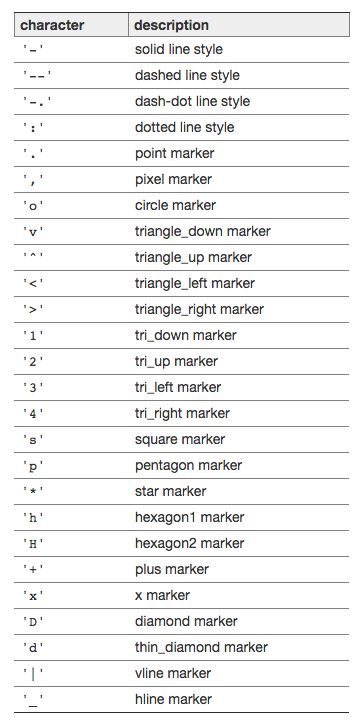
\includegraphics{style.png}

\begin{enumerate}
\def\labelenumi{\arabic{enumi}.}
\setcounter{enumi}{1}
\tightlist
\item
  顏色
\end{enumerate}

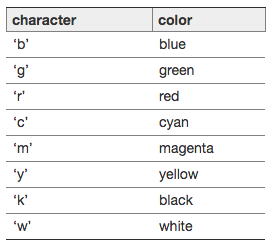
\includegraphics{color.png}

    \begin{Verbatim}[commandchars=\\\{\}]
{\color{incolor}In [{\color{incolor}3}]:} \PY{n}{x\PYZus{}list} \PY{o}{=} \PY{p}{[}\PY{l+m+mi}{1}\PY{p}{,} \PY{l+m+mi}{2}\PY{p}{,} \PY{l+m+mi}{3}\PY{p}{,} \PY{l+m+mi}{4}\PY{p}{]}
        \PY{n}{y\PYZus{}list} \PY{o}{=} \PY{p}{[}\PY{l+m+mi}{1}\PY{p}{,} \PY{l+m+mi}{2}\PY{p}{,} \PY{l+m+mi}{6}\PY{p}{,} \PY{l+m+mi}{8}\PY{p}{]}
        \PY{c+c1}{\PYZsh{} dash\PYZhy{}line + green color}
        \PY{n}{plt}\PY{o}{.}\PY{n}{plot}\PY{p}{(}\PY{n}{x\PYZus{}list}\PY{p}{,} \PY{n}{y\PYZus{}list}\PY{p}{,} \PY{l+s+s2}{\PYZdq{}}\PY{l+s+s2}{\PYZhy{}\PYZhy{}g}\PY{l+s+s2}{\PYZdq{}}\PY{p}{)}
        \PY{n}{plt}\PY{o}{.}\PY{n}{show}\PY{p}{(}\PY{p}{)}
\end{Verbatim}


    \begin{center}
    \adjustimage{max size={0.9\linewidth}{0.9\paperheight}}{output_4_0.png}
    \end{center}
    { \hspace*{\fill} \\}
    
    \hypertarget{ux52a0ux4e0aux6a19ux7c64}{%
\subsection{加上標籤}\label{ux52a0ux4e0aux6a19ux7c64}}

\begin{enumerate}
\def\labelenumi{\arabic{enumi}.}
\tightlist
\item
  在plot的時候加上參數label
\item
  記得要用legend放在對的位置上,不然一樣看不到
\item
  可以用xlabel()和ylabel()加上x軸標籤和y軸標籤
\end{enumerate}

    \begin{Verbatim}[commandchars=\\\{\}]
{\color{incolor}In [{\color{incolor}4}]:} \PY{n}{x\PYZus{}list} \PY{o}{=} \PY{p}{[}\PY{l+m+mi}{1}\PY{p}{,} \PY{l+m+mi}{2}\PY{p}{,} \PY{l+m+mi}{3}\PY{p}{,} \PY{l+m+mi}{4}\PY{p}{]}
        \PY{n}{y\PYZus{}list} \PY{o}{=} \PY{p}{[}\PY{l+m+mi}{1}\PY{p}{,} \PY{l+m+mi}{2}\PY{p}{,} \PY{l+m+mi}{6}\PY{p}{,} \PY{l+m+mi}{8}\PY{p}{]}
        \PY{c+c1}{\PYZsh{} dash\PYZhy{}line + green color}
        \PY{n}{plt}\PY{o}{.}\PY{n}{plot}\PY{p}{(}\PY{n}{x\PYZus{}list}\PY{p}{,} \PY{n}{y\PYZus{}list}\PY{p}{,} \PY{l+s+s2}{\PYZdq{}}\PY{l+s+s2}{\PYZhy{}\PYZhy{}g}\PY{l+s+s2}{\PYZdq{}}\PY{p}{,} \PY{n}{label} \PY{o}{=} \PY{l+s+s2}{\PYZdq{}}\PY{l+s+s2}{random}\PY{l+s+s2}{\PYZdq{}}\PY{p}{)}
        \PY{n}{plt}\PY{o}{.}\PY{n}{legend}\PY{p}{(}\PY{n}{loc} \PY{o}{=} \PY{l+s+s2}{\PYZdq{}}\PY{l+s+s2}{lower right}\PY{l+s+s2}{\PYZdq{}}\PY{p}{)}
        \PY{n}{plt}\PY{o}{.}\PY{n}{xlabel}\PY{p}{(}\PY{l+s+s2}{\PYZdq{}}\PY{l+s+s2}{\PYZsh{} of x}\PY{l+s+s2}{\PYZdq{}}\PY{p}{)}
        \PY{n}{plt}\PY{o}{.}\PY{n}{ylabel}\PY{p}{(}\PY{l+s+s2}{\PYZdq{}}\PY{l+s+s2}{\PYZsh{} of y}\PY{l+s+s2}{\PYZdq{}}\PY{p}{)}
        \PY{n}{plt}\PY{o}{.}\PY{n}{show}\PY{p}{(}\PY{p}{)}
\end{Verbatim}


    \begin{center}
    \adjustimage{max size={0.9\linewidth}{0.9\paperheight}}{output_6_0.png}
    \end{center}
    { \hspace*{\fill} \\}
    
    \hypertarget{ux76e1ux91cfux4e0dux8981-ux4e2dux6587ux986fux793a}{%
\subsection{(盡量不要)
中文顯示}\label{ux76e1ux91cfux4e0dux8981-ux4e2dux6587ux986fux793a}}

\begin{enumerate}
\def\labelenumi{\arabic{enumi}.}
\tightlist
\item
  Matplotlib預設只有外文字體,對於外文字體的顯示也比較漂亮一點
\item
  如果你真的萬不得已,想要使用中文字體來顯示,要特別將預設的字體修改成中文字體
\end{enumerate}

\hypertarget{ux4f7fux7528ux5b57ux9ad4}{%
\subsection{使用字體}\label{ux4f7fux7528ux5b57ux9ad4}}

STHeiti(蘋果黑體):
Mac內建字型,由於這裡OS是使用Mac,所以我選擇了Mac內建的字型

    \begin{Verbatim}[commandchars=\\\{\}]
{\color{incolor}In [{\color{incolor}5}]:} \PY{k+kn}{import} \PY{n+nn}{matplotlib}
        \PY{n}{matplotlib}\PY{o}{.}\PY{n}{rcParams}\PY{p}{[}\PY{l+s+s1}{\PYZsq{}}\PY{l+s+s1}{font.sans\PYZhy{}serif}\PY{l+s+s1}{\PYZsq{}}\PY{p}{]} \PY{o}{=} \PY{l+s+s1}{\PYZsq{}}\PY{l+s+s1}{STHeiti}\PY{l+s+s1}{\PYZsq{}}
        \PY{n}{x\PYZus{}list} \PY{o}{=} \PY{p}{[}\PY{l+m+mi}{1}\PY{p}{,} \PY{l+m+mi}{2}\PY{p}{,} \PY{l+m+mi}{3}\PY{p}{,} \PY{l+m+mi}{4}\PY{p}{]}
        \PY{n}{y\PYZus{}list} \PY{o}{=} \PY{p}{[}\PY{l+m+mi}{1}\PY{p}{,} \PY{l+m+mi}{2}\PY{p}{,} \PY{l+m+mi}{6}\PY{p}{,} \PY{l+m+mi}{8}\PY{p}{]}
        \PY{c+c1}{\PYZsh{} dash\PYZhy{}dot + blue color}
        \PY{n}{plt}\PY{o}{.}\PY{n}{plot}\PY{p}{(}\PY{n}{x\PYZus{}list}\PY{p}{,} \PY{n}{y\PYZus{}list}\PY{p}{,} \PY{l+s+s2}{\PYZdq{}}\PY{l+s+s2}{\PYZhy{}.b}\PY{l+s+s2}{\PYZdq{}}\PY{p}{,} \PY{n}{label} \PY{o}{=} \PY{l+s+s2}{\PYZdq{}}\PY{l+s+s2}{random}\PY{l+s+s2}{\PYZdq{}}\PY{p}{)}
        \PY{n}{plt}\PY{o}{.}\PY{n}{legend}\PY{p}{(}\PY{n}{loc} \PY{o}{=} \PY{l+s+s2}{\PYZdq{}}\PY{l+s+s2}{lower right}\PY{l+s+s2}{\PYZdq{}}\PY{p}{)}
        \PY{n}{plt}\PY{o}{.}\PY{n}{xlabel}\PY{p}{(}\PY{l+s+s2}{\PYZdq{}}\PY{l+s+s2}{x的數目}\PY{l+s+s2}{\PYZdq{}}\PY{p}{)}
        \PY{n}{plt}\PY{o}{.}\PY{n}{ylabel}\PY{p}{(}\PY{l+s+s2}{\PYZdq{}}\PY{l+s+s2}{y的數目}\PY{l+s+s2}{\PYZdq{}}\PY{p}{)}
        \PY{n}{plt}\PY{o}{.}\PY{n}{show}\PY{p}{(}\PY{p}{)}
\end{Verbatim}


    \begin{center}
    \adjustimage{max size={0.9\linewidth}{0.9\paperheight}}{output_8_0.png}
    \end{center}
    { \hspace*{\fill} \\}
    
    \hypertarget{ux9435ux9054ux5c3cux865f-seaborn}{%
\subsection{✔ 鐵達尼號 +
Seaborn}\label{ux9435ux9054ux5c3cux865f-seaborn}}

\begin{enumerate}
\def\labelenumi{\arabic{enumi}.}
\tightlist
\item
  使用Pandas先將鐵達尼號的資料讀取出來
\item
  Survied欄位: 0代表無法倖存的乘客 1代表倖存的乘客
\item
  以下是每個欄位代表的意思 
\end{enumerate}

    \begin{Verbatim}[commandchars=\\\{\}]
{\color{incolor}In [{\color{incolor}6}]:} \PY{k+kn}{import} \PY{n+nn}{pandas} \PY{k}{as} \PY{n+nn}{pd}
        \PY{c+c1}{\PYZsh{} 為了顯示的漂亮, 我刻意的把印出來的row只顯示20個和column只顯示十個, 大家練習的時候可以去掉下面兩行}
        \PY{n}{pd}\PY{o}{.}\PY{n}{set\PYZus{}option}\PY{p}{(}\PY{l+s+s1}{\PYZsq{}}\PY{l+s+s1}{display.max\PYZus{}rows}\PY{l+s+s1}{\PYZsq{}}\PY{p}{,} \PY{l+m+mi}{20}\PY{p}{)}
        \PY{n}{pd}\PY{o}{.}\PY{n}{set\PYZus{}option}\PY{p}{(}\PY{l+s+s1}{\PYZsq{}}\PY{l+s+s1}{display.max\PYZus{}columns}\PY{l+s+s1}{\PYZsq{}}\PY{p}{,} \PY{l+m+mi}{10}\PY{p}{)}
        
        \PY{n}{df} \PY{o}{=} \PY{n}{pd}\PY{o}{.}\PY{n}{read\PYZus{}csv}\PY{p}{(}\PY{l+s+s2}{\PYZdq{}}\PY{l+s+s2}{train.csv}\PY{l+s+s2}{\PYZdq{}}\PY{p}{,} \PY{n}{encoding} \PY{o}{=} \PY{l+s+s2}{\PYZdq{}}\PY{l+s+s2}{utf\PYZhy{}8}\PY{l+s+s2}{\PYZdq{}}\PY{p}{)}
        \PY{n}{df}
\end{Verbatim}


\begin{Verbatim}[commandchars=\\\{\}]
{\color{outcolor}Out[{\color{outcolor}6}]:}      PassengerId  Survived  Pclass  \textbackslash{}
        0              1         0       3   
        1              2         1       1   
        2              3         1       3   
        3              4         1       1   
        4              5         0       3   
        5              6         0       3   
        6              7         0       1   
        7              8         0       3   
        8              9         1       3   
        9             10         1       2   
        ..           {\ldots}       {\ldots}     {\ldots}   
        881          882         0       3   
        882          883         0       3   
        883          884         0       2   
        884          885         0       3   
        885          886         0       3   
        886          887         0       2   
        887          888         1       1   
        888          889         0       3   
        889          890         1       1   
        890          891         0       3   
        
                                                          Name     Sex    {\ldots}     \textbackslash{}
        0                              Braund, Mr. Owen Harris    male    {\ldots}      
        1    Cumings, Mrs. John Bradley (Florence Briggs Th{\ldots}  female    {\ldots}      
        2                               Heikkinen, Miss. Laina  female    {\ldots}      
        3         Futrelle, Mrs. Jacques Heath (Lily May Peel)  female    {\ldots}      
        4                             Allen, Mr. William Henry    male    {\ldots}      
        5                                     Moran, Mr. James    male    {\ldots}      
        6                              McCarthy, Mr. Timothy J    male    {\ldots}      
        7                       Palsson, Master. Gosta Leonard    male    {\ldots}      
        8    Johnson, Mrs. Oscar W (Elisabeth Vilhelmina Berg)  female    {\ldots}      
        9                  Nasser, Mrs. Nicholas (Adele Achem)  female    {\ldots}      
        ..                                                 {\ldots}     {\ldots}    {\ldots}      
        881                                 Markun, Mr. Johann    male    {\ldots}      
        882                       Dahlberg, Miss. Gerda Ulrika  female    {\ldots}      
        883                      Banfield, Mr. Frederick James    male    {\ldots}      
        884                             Sutehall, Mr. Henry Jr    male    {\ldots}      
        885               Rice, Mrs. William (Margaret Norton)  female    {\ldots}      
        886                              Montvila, Rev. Juozas    male    {\ldots}      
        887                       Graham, Miss. Margaret Edith  female    {\ldots}      
        888           Johnston, Miss. Catherine Helen "Carrie"  female    {\ldots}      
        889                              Behr, Mr. Karl Howell    male    {\ldots}      
        890                                Dooley, Mr. Patrick    male    {\ldots}      
        
             Parch            Ticket     Fare Cabin  Embarked  
        0        0         A/5 21171   7.2500   NaN         S  
        1        0          PC 17599  71.2833   C85         C  
        2        0  STON/O2. 3101282   7.9250   NaN         S  
        3        0            113803  53.1000  C123         S  
        4        0            373450   8.0500   NaN         S  
        5        0            330877   8.4583   NaN         Q  
        6        0             17463  51.8625   E46         S  
        7        1            349909  21.0750   NaN         S  
        8        2            347742  11.1333   NaN         S  
        9        0            237736  30.0708   NaN         C  
        ..     {\ldots}               {\ldots}      {\ldots}   {\ldots}       {\ldots}  
        881      0            349257   7.8958   NaN         S  
        882      0              7552  10.5167   NaN         S  
        883      0  C.A./SOTON 34068  10.5000   NaN         S  
        884      0   SOTON/OQ 392076   7.0500   NaN         S  
        885      5            382652  29.1250   NaN         Q  
        886      0            211536  13.0000   NaN         S  
        887      0            112053  30.0000   B42         S  
        888      2        W./C. 6607  23.4500   NaN         S  
        889      0            111369  30.0000  C148         C  
        890      0            370376   7.7500   NaN         Q  
        
        [891 rows x 12 columns]
\end{Verbatim}
            
    \hypertarget{importux51fdux5f0fux5eabux4ee5ux53caux5229ux7528notebook}{%
\subsection{Import函式庫以及利用Notebook}\label{importux51fdux5f0fux5eabux4ee5ux53caux5229ux7528notebook}}

\begin{enumerate}
\def\labelenumi{\arabic{enumi}.}
\tightlist
\item
  由於Seaborn是基於Matplotlib的函式庫,所以正常寫法下,你一樣得在最後一行加上plt.show()印出圖形
\item
  在Jupyter
  Notebook裡使用的時候其實可以透過他提供給我們的簡便工具來簡化我們使用
\item
  (重要,且只有Notebook可以用) 加上\%matplotlib
  inline這行的話,你就可以在每次做圖的時候少打plt.show()
\end{enumerate}

    \begin{Verbatim}[commandchars=\\\{\}]
{\color{incolor}In [{\color{incolor}7}]:} \PY{c+c1}{\PYZsh{} 大家這裡習慣給他改名成sns}
        \PY{k+kn}{import} \PY{n+nn}{seaborn} \PY{k}{as} \PY{n+nn}{sns}
        \PY{c+c1}{\PYZsh{} 這行只有在Jupyter Notebook可以使用}
        \PY{o}{\PYZpc{}}\PY{k}{matplotlib} inline
        \PY{c+c1}{\PYZsh{} sns每次會跳出remove\PYZus{}na的warning}
        \PY{c+c1}{\PYZsh{} 我為了頁面的美化 不讓warning印出,但讀者不一定要過濾掉}
        \PY{k+kn}{import} \PY{n+nn}{warnings}
        \PY{n}{warnings}\PY{o}{.}\PY{n}{filterwarnings}\PY{p}{(}\PY{l+s+s1}{\PYZsq{}}\PY{l+s+s1}{ignore}\PY{l+s+s1}{\PYZsq{}}\PY{p}{)}
\end{Verbatim}


    \hypertarget{ux6578ux91cfux5716}{%
\subsection{✔ 數量圖}\label{ux6578ux91cfux5716}}

\begin{enumerate}
\def\labelenumi{\arabic{enumi}.}
\tightlist
\item
  數量圖是在類別做圖的時候一個很好用的圖示工具,統計各個類別分別有多少數量
\item
  使用seaborn.countplot,我們通常選擇只設置其中一軸,另一軸就是數量
\item
  你可以藉由palette這個參數來選擇一下你喜歡的整體色系
\item
  palette:
  https://seaborn.pydata.org/generated/seaborn.color\_palette.html\#seaborn.color\_palette
\end{enumerate}

    \begin{Verbatim}[commandchars=\\\{\}]
{\color{incolor}In [{\color{incolor}8}]:} \PY{c+c1}{\PYZsh{} 針對一個類別做數量圖,由於我們inline了matplotlib,所以不需要plt.show()}
        \PY{c+c1}{\PYZsh{} 設置x軸的往上長的長條圖}
        \PY{n}{sns}\PY{o}{.}\PY{n}{countplot}\PY{p}{(}\PY{n}{x} \PY{o}{=} \PY{n}{df}\PY{p}{[}\PY{l+s+s2}{\PYZdq{}}\PY{l+s+s2}{Survived}\PY{l+s+s2}{\PYZdq{}}\PY{p}{]}\PY{p}{,} \PY{n}{palette} \PY{o}{=} \PY{l+s+s2}{\PYZdq{}}\PY{l+s+s2}{Reds\PYZus{}d}\PY{l+s+s2}{\PYZdq{}}\PY{p}{)}
\end{Verbatim}


\begin{Verbatim}[commandchars=\\\{\}]
{\color{outcolor}Out[{\color{outcolor}8}]:} <matplotlib.axes.\_subplots.AxesSubplot at 0x114c73128>
\end{Verbatim}
            
    \begin{center}
    \adjustimage{max size={0.9\linewidth}{0.9\paperheight}}{output_14_1.png}
    \end{center}
    { \hspace*{\fill} \\}
    
    \begin{Verbatim}[commandchars=\\\{\}]
{\color{incolor}In [{\color{incolor}9}]:} \PY{c+c1}{\PYZsh{} 針對一個類別做數量圖,由於我們inline了matplotlib,所以不需要plt.show()}
        \PY{c+c1}{\PYZsh{} 設置y軸的往右長的長條圖}
        \PY{c+c1}{\PYZsh{} 畫出各艙等的人數}
        \PY{n}{sns}\PY{o}{.}\PY{n}{countplot}\PY{p}{(}\PY{n}{y} \PY{o}{=} \PY{n}{df}\PY{p}{[}\PY{l+s+s2}{\PYZdq{}}\PY{l+s+s2}{Pclass}\PY{l+s+s2}{\PYZdq{}}\PY{p}{]}\PY{p}{,} \PY{n}{palette} \PY{o}{=} \PY{l+s+s2}{\PYZdq{}}\PY{l+s+s2}{Greens\PYZus{}d}\PY{l+s+s2}{\PYZdq{}}\PY{p}{)}
\end{Verbatim}


\begin{Verbatim}[commandchars=\\\{\}]
{\color{outcolor}Out[{\color{outcolor}9}]:} <matplotlib.axes.\_subplots.AxesSubplot at 0x114c9d208>
\end{Verbatim}
            
    \begin{center}
    \adjustimage{max size={0.9\linewidth}{0.9\paperheight}}{output_15_1.png}
    \end{center}
    { \hspace*{\fill} \\}
    
    \begin{Verbatim}[commandchars=\\\{\}]
{\color{incolor}In [{\color{incolor}10}]:} \PY{c+c1}{\PYZsh{} 結合上面兩個,把一個區域的長條加入第二個特徵,統計第二個特徵+第一個特徵的數目}
         \PY{c+c1}{\PYZsh{} hue裡面放的就是第二個特徵}
         \PY{c+c1}{\PYZsh{} 你找到了其中一個相關性: 第三艙等的存活率稍微低了一點}
         \PY{n}{sns}\PY{o}{.}\PY{n}{countplot}\PY{p}{(}\PY{n}{x} \PY{o}{=} \PY{n}{df}\PY{p}{[}\PY{l+s+s2}{\PYZdq{}}\PY{l+s+s2}{Survived}\PY{l+s+s2}{\PYZdq{}}\PY{p}{]}\PY{p}{,} \PY{n}{hue} \PY{o}{=} \PY{n}{df}\PY{p}{[}\PY{l+s+s2}{\PYZdq{}}\PY{l+s+s2}{Pclass}\PY{l+s+s2}{\PYZdq{}}\PY{p}{]}\PY{p}{,} \PY{n}{palette} \PY{o}{=} \PY{l+s+s2}{\PYZdq{}}\PY{l+s+s2}{Blues\PYZus{}d}\PY{l+s+s2}{\PYZdq{}}\PY{p}{)}
\end{Verbatim}


\begin{Verbatim}[commandchars=\\\{\}]
{\color{outcolor}Out[{\color{outcolor}10}]:} <matplotlib.axes.\_subplots.AxesSubplot at 0x114d068d0>
\end{Verbatim}
            
    \begin{center}
    \adjustimage{max size={0.9\linewidth}{0.9\paperheight}}{output_16_1.png}
    \end{center}
    { \hspace*{\fill} \\}
    
    \hypertarget{facetgridux7db2ux683cux5716-ux5206ux5e03ux5716}{%
\subsection{✔ FacetGrid網格圖 +
分布圖}\label{facetgridux7db2ux683cux5716-ux5206ux5e03ux5716}}

\hypertarget{facetgridux7db2ux683cux5716}{%
\subsubsection{FacetGrid網格圖}\label{facetgridux7db2ux683cux5716}}

\begin{enumerate}
\def\labelenumi{\arabic{enumi}.}
\tightlist
\item
  FacetGrid網格圖是你可以固定變數的一種圖形,你設定的欄位會把所有可能的值拿出來,變出這麼多圖出來
\item
  可以設定row和col,你的圖的數量就等於 row可能數 * col可能數
\item
  使用FacetGrid來創造,記得最後要給你的每個圖一個畫圖方式(ex. 分布圖)
\item
  FacetGrid是一個跟pandas非常友善的設計,你可以將DataFrame直接丟給第一個參數
\item
  使用FacetGrid的主因之一是我們要做出分布圖(x軸是連續的),但連續的東西我們沒辦法像上面的countplot分成三條來看,會看不出連續的趨勢
\end{enumerate}

    \begin{Verbatim}[commandchars=\\\{\}]
{\color{incolor}In [{\color{incolor}11}]:} \PY{c+c1}{\PYZsh{} 對每一個網格裡的圖做下面的初始化}
         \PY{c+c1}{\PYZsh{} 由於剛剛已經設定完data, 這裡直接給他欄位的名稱當x軸即可}
         \PY{n}{fg} \PY{o}{=} \PY{n}{sns}\PY{o}{.}\PY{n}{FacetGrid}\PY{p}{(}\PY{n}{df}\PY{p}{,} \PY{n}{col} \PY{o}{=} \PY{l+s+s2}{\PYZdq{}}\PY{l+s+s2}{Survived}\PY{l+s+s2}{\PYZdq{}}\PY{p}{)}
\end{Verbatim}


    \begin{center}
    \adjustimage{max size={0.9\linewidth}{0.9\paperheight}}{output_18_0.png}
    \end{center}
    { \hspace*{\fill} \\}
    
    \hypertarget{distplotux5206ux5e03ux5716}{%
\subsubsection{DistPlot分布圖}\label{distplotux5206ux5e03ux5716}}

\begin{enumerate}
\def\labelenumi{\arabic{enumi}.}
\tightlist
\item
  通常我們使用了網格圖以後,我們需要對每個圖初始化,我們常用的就是分佈圖
\item
  分布圖要傳入一個一個維度的群集,ex. 一個Series
\item
  他會把你傳入的一維群集轉換成x軸的區間
\item
  跟Countplot一個很大的不同是我們的x軸是連續的,不是分類型的
\item
  你可以給你的分布圖一個顏色: https://matplotlib.org/users/colors.html
\end{enumerate}

    \begin{Verbatim}[commandchars=\\\{\}]
{\color{incolor}In [{\color{incolor}12}]:} \PY{n}{fg} \PY{o}{=} \PY{n}{sns}\PY{o}{.}\PY{n}{FacetGrid}\PY{p}{(}\PY{n}{df}\PY{p}{,} \PY{n}{col} \PY{o}{=} \PY{l+s+s2}{\PYZdq{}}\PY{l+s+s2}{Survived}\PY{l+s+s2}{\PYZdq{}}\PY{p}{)}
         \PY{n}{fg}\PY{o}{.}\PY{n}{map}\PY{p}{(}\PY{n}{sns}\PY{o}{.}\PY{n}{distplot}\PY{p}{,} \PY{l+s+s1}{\PYZsq{}}\PY{l+s+s1}{Age}\PY{l+s+s1}{\PYZsq{}}\PY{p}{,} \PY{n}{color} \PY{o}{=} \PY{l+s+s2}{\PYZdq{}}\PY{l+s+s2}{yellowgreen}\PY{l+s+s2}{\PYZdq{}}\PY{p}{,} \PY{n}{kde} \PY{o}{=} \PY{k+kc}{True}\PY{p}{)}
\end{Verbatim}


\begin{Verbatim}[commandchars=\\\{\}]
{\color{outcolor}Out[{\color{outcolor}12}]:} <seaborn.axisgrid.FacetGrid at 0x114f83ef0>
\end{Verbatim}
            
    \begin{center}
    \adjustimage{max size={0.9\linewidth}{0.9\paperheight}}{output_20_1.png}
    \end{center}
    { \hspace*{\fill} \\}
    

    % Add a bibliography block to the postdoc
    
    
    
    \end{document}
